% -*- coding: UTF-8 -*-
% hurlex-chapt3.tex
% hurlex 开发文档 第3章内容

\section{裸机上运行的 Hello OS Kernel}

\par 不知道前两章的文字大家看烦了没有?除了第一章还有简单的动手任务之外,之后都是无聊的文字描述了。嘿嘿,必要的铺垫还是得有的,\allowbreak
虽然以后大段的概念依然少不了,但是从本章开始,我们就要开始进入实战阶段了。

\subsection{Makefile和ld脚本的简单解释}

\par 我们先简单的解释一下之前的Makefile和ld链接脚本的一些字段,如果你已经掌握了,那大致浏览下就可以跳过这段文字了。

\par 先来看Makefile中关于gcc编译参数的这一行:

\begin{Verbatim}[frame=single]
  C_FLAGS = -c -Wall -m32 -ggdb -gstabs+ -nostdinc -fno-builtin
		-fno-stack-protector -I include
\end{Verbatim}

\par 我们只解释以下重要的几个参数:
\begin{itemize}
	\item -m32 是生成32位代码,这样的话我们的开发环境也可以使用64位的Linux系统。
	\item -ggdb 和-gstabs+ 是添加相关的调试信息,调试对后期的排错很重要。
	\item -nostdinc 是不包含C语言的标准库里的头文件。\allowbreak
		\footnote{尽管可以使用C语言进行开发,但是几乎所有C语言的库函数和我们告别了。因为那些库函数都是在特\allowbreak
		定操作系统平台之上的实现,而我们要做的正是实现这样一个平台,所以想用C语言库的话就需要自己实现了。}
	\item -fno-builtin 是要求gcc不主动使用自己的内建函数,除非显式声明。
		\footnote{gcc有很多内建函数用来替换一些C语言的库函数以提升效率,比如把只有一个字符串参数的printf函数替换为puts函数。}
	\item -fno-stack-protector 是不使用栈保护等检测。
\end{itemize}

\par 接着是ld链接命令的参数:
\begin{Verbatim}[frame=single]
  LD_FLAGS = -T scripts/kernel.ld -m elf_i386 -nostblib
\end{Verbatim}

\begin{itemize}
	\item -T scripts/kernel.ld 是使用我们自己的链接器脚本。
	\item -m elf\_i386 是生成i386平台下的ELF格式的可执行文件,这是Linux下的可执行文件格式。
	\item -nostdlib 是不链接C语言的标准库,原因上文已经交代过了。
\end{itemize}

\par 接下来讨论链接器脚本。

\par 我们知道一个可执行的文件大致由代码段和数据段组成,但是操作系统怎么正确加载它呢?事实上可执行文件有义务向操作系统提供\allowbreak
代码段和数据段位置等信息,以便操作系统正确找到它的代码段和数据段并加载执行。通常这个信息被统一组织放置在可执行文件的头部区域。\allowbreak
不同的操作系统中自然就设计了不同的组织方式,比如Linux常见的ELF(Executable and Linkable Format,可执行链接格式)格式,\allowbreak
windows下常见的PE(Portable Executable,可移植的可执行文件)格式都是。\allowbreak
\footnote{其实Linux下的ELF格式和Windows下的PE格式都是COFF(Common Object File Format,通用对象文件格式)\allowbreak
格式的一个变种。}而ld支持很多种链接格式,我们可以在参数里指定。那为何选择ELF格式呢?原因很简单,因为GRUB可以检测\allowbreak
识别出ELF格式的可执行文件,并且能找到相关的代码段和数据段的位置信息,从而正确的把我们的内核加载到正确的位置上去。

\par 看懂了这个Makefile和链接器脚本,我们就向成功迈出了一大步了。大家还记得上一章谈过的GRUB Multiboot标准吗?\allowbreak
只要按照标准生成规范的Multiboot引导信息,同时使用标准的ELF格式,GRUB就能把我们的内核正确的加载和执行了。

\par 说了这么多,现在大家对计算机从加电到执行我们的内核的过程有概念了吧?如果感觉还是很模糊也不要紧,毕竟第一次接触\allowbreak
这些东西难免需要时间消化。随着我们研究的展开,相信你会越来越清晰的。\allowbreak
\footnote{不知道我在前面说的编译链接的过程和可执行文件的结果大家了解过没?没有的话请回去看明白了再回来。因为这直接\allowbreak
关系到你对后续章节的理解程度。如果上面的描述你看的是稀里糊涂的话,还请你先学习了相关的知识背景之后再继续和我做下去,\allowbreak
否则稀里糊涂的玩下去意义真的不是很大,毕竟这不是用来应付的家庭作业。}

\subsection{启动镜像的制作}

\par 解决了理论上的问题之后,我们来解决一个现实的问题。这个问题是,这个小内核放在哪里?虚拟机是它运行的场所,那么虚拟\allowbreak
磁盘自然就是安放内核的选择了。不过我们这次不选择硬盘,而是选择已经几乎消失殆尽的1.44MB的软盘。为什么?说实话是因为比较简单。\allowbreak
\footnote{这个答案有点囧是不是?其实从一开始到现在,我们已经为了求简做了很多妥协了,从精简的描述到通俗的概念解释,再到使用\allowbreak
现成的bootloader程序,现在又使用简单的外部存储。这么做一是我自己确实水平很有限,二是这篇文档的定位是初学者,不能过于复杂\allowbreak
,所以还请大家多多担待。}

\par 在Linux下制作一个1.44MB软盘的技术太简单了,甚至dd命令也可以做一个出来。\allowbreak
\footnote{老规矩,大家自己上Google搜索,学会自己探索是很重要的。}不过在这个软盘镜像上安装一个GRUB稍有难度,\allowbreak
所以大家直接可以使用我提供的已经安装好了GRUB的软盘镜像。\allowbreak
\footnote{这个软盘镜像的作者是Jamesm先生,再次表示感谢。不过建议有基础的读者去Google检索相关资料,自己做一个出来。}

\par 大家准备好镜像了吗?OK!万事俱备,只欠代码了。让我们开始最激动人心的探索吧!
\par 抱歉,我又得打断一下。因为必须引入一个新的术语名词——文件系统。什么是文件系统呢?其实简单的说,这里所谓\allowbreak
的文件系统指的是操作系统用于明确磁盘或分区上的文件存储的方法和数据结构,即在磁盘上组织文件的方法。如果把这个1.44MB\allowbreak
的软盘可以看做一个巨大的数组,那么每个数组成员都是一个扇区,拥有512字节的存储单元。现在需要往这个软盘上写入文件,那么自然\allowbreak
需要一套合适的管理规则,否则的话岂不是全乱套了?就和这篇文档一样,不同的章节被划分在不同的位置,同时在最前面有所有章节\allowbreak
的目录,这就是一种对信息的组织方式,文件系统也不过是这么一套组织策略罢了。\allowbreak
\footnote{当然,这里只是通俗的解释了文件系统的基本概念,其实设计一个优秀的文件系统是一件并不容易的事情,需要考虑到很多因素。}

\par 考虑到兼容因素,自然是选择目前使用的比较广泛的文件系统了,这样的话也便于我们对软盘里面存储的文件进行管理操作。\allowbreak
\footnote{这个理由听起来不错。其实弱弱的说一句,还有一个原因是我自己目前没有设计一个文件系统的能力。嘘~这是秘密,\allowbreak
千万别说出去。}那么使用什么文件系统呢?软盘一般使用的是FAT12文件系统,所以我们也就不标新立异了。这个文件系统也很\allowbreak
简单,后期大家有兴趣的话甚至可以在我们的内核里实现能处理这个文件系统的代码。至于FAT12文件系统的资料也很多,我就不详细说了。\allowbreak
\footnote{经过前面的几次去Google检索,相信大家现在搜索资料的水平强了不少吧?那就再接再厉,自己简单浏览下FAT12的一些资料吧。}\allowbreak
GRUB支持从很多常见的文件系统中去读取和载入内核文件,当然也包括我们使用的FAT12格式。我们在自己开发使用的Linux系统上很容易就\allowbreak
可以挂载和读写这个虚拟软盘里的文件,这给开发带来了极大的便利。我们经常做的事就是拷贝编译好的内核进去,然后在虚拟机\allowbreak
运行。另外这个虚拟软盘文件里还有GRUB和它的配置文件,我提供的软盘镜像里安装的是一个很早的GRUB版本,它的配置文件简单到\allowbreak
一看就懂。\footnote{本着够用就好的原则,较早的GRU版本就完全满足我们的需求了,而新版的GRUB配置起来比较麻烦。}\allowbreak
所以大家完全可以自己看着修改。\footnote{其实也没有什么需要改的,主要是GRUB载入的内核文件名。我的内核名叫做hx\_kernel,\allowbreak
如果你嫌麻烦,和我叫一个名字就不用修改GRUB配置了。}

\subsection{内核的入口和初始化}

\par 前期的铺垫到这里就告一段落了,下面我们开始编码工作吧。

\par 代码从什么函数开始执行呢?如果你记忆力足够好的话你会记得ld链接脚本里面的一行文字:

\begin{Verbatim}[frame=single]
  ENTRY(start)
\end{Verbatim}

\par 这就意味着我们告诉了ld链接器入口函数是start,所以代码从start函数开始。\allowbreak
\footnote{入口可以自由定义,只要在ld链接脚本里修改就可以。要知道我们现在是在写一个操作系统内核,在这里我们几乎可以定制一切。}

\par 大家先来一起围观下入口部分的代码全貌:

\begin{lstlisting}[language = {[x86masm]Assembler}, label = boot/boot.s, caption = boot/boot.s]
; ----------------------------------------------------------------
;
; 	boot.s -- 内核从这里开始
;
; ----------------------------------------------------------------

; Multiboot 魔数,由规范决定的
MBOOT_HEADER_MAGIC 	equ 	0x1BADB002

; 0 号位表示所有的引导模块将按页(4KB)边界对齐
MBOOT_PAGE_ALIGN 	equ 	1 << 0

; 1 号位通过 Multiboot 信息结构的 mem_* 域包括可用内存的信息
; (告诉GRUB把内存空间的信息包含在Mutiboot信息结构中)
MBOOT_MEM_INFO 		equ 	1 << 1    

; 定义我们使用的 Multiboot 的标记
MBOOT_HEADER_FLAGS 	equ 	MBOOT_PAGE_ALIGN | MBOOT_MEM_INFO

; 域checksum是一个32位的无符号值,当与其他的magic域(也就是magic和flags)
; 相加时,要求其结果必须是32位的无符号值 0 (即magic+flags+checksum = 0)
MBOOT_CHECKSUM 		equ 	-(MBOOT_HEADER_MAGIC+MBOOT_HEADER_FLAGS)

; 符合Multiboot规范的 OS 映象需要这样一个 magic Multiboot 头
; Multiboot 头的分布必须如下表所示:
; ----------------------------------------------------------
; 偏移量  类型  域名        备注
;
;   0     u32   magic       必需
;   4     u32   flags       必需 
;   8     u32   checksum    必需 
;
; 我们只使用到这些就够了,更多的详细说明请参阅 GNU 相关文档
;-----------------------------------------------------------

[BITS 32]  	; 所有代码以 32-bit 的方式编译

section .text 	; 代码段从这里开始

; 在代码段的起始位置设置符合 Multiboot 规范的标记

dd MBOOT_HEADER_MAGIC 	; GRUB 会通过这个魔数判断该映像是否支持
dd MBOOT_HEADER_FLAGS   ; GRUB 的一些加载时选项,其详细注释在定义处
dd MBOOT_CHECKSUM       ; 检测数值,其含义在定义处

[GLOBAL start] 		; 内核代码入口,此处提供该声明给 ld 链接器
[EXTERN kern_entry] 	; 声明内核 C 代码的入口函数

start:
	cli  		; 此时还没有设置好保护模式的中断处理
			; 所以必须关闭中断
	mov esp, stack  ; 设置内核栈地址
	push ebx 	; 调用内核 main 函数的参数
	mov ebp, 0 	; 帧指针修改为 0
	call kern_entry	; 调用内核入口函数
stop:
	hlt 		; 停机指令,什么也不做,可以降低 CPU 功耗
	jmp stop 	; 到这里结束,关机什么的后面再说
	
[GLOBAL stack]
section .bss 		; 未初始化的数据段从这里开始
	resb 32768 	; 这里作为内核栈
stack:
\end{lstlisting} 

\par 我们简单的介绍下这段代码做的事情。
\par 首先是一些宏定义,定义了Multiboot标准的魔数和几个标识,GRUB会读取这些信息以判断我们的意图。真正的代码是从\allowbreak
39行以后开始的,首先我们在代码段的入口位置之前定义了几个Multiboot规范要求的配置信息,其实也就是3个4字节变量。我们通过\allowbreak
这几个变量告诉了GRUB我们要求它提供可用内存的信息,而且要求内核中所有的段在内存里按照4KB进行对齐。\allowbreak
\footnote{后面谈到分页后你就明白这里的4KB对齐之类的含义了,暂时先按照我的要求做吧。}紧接着就是我们内核的入口函数\allowbreak
start了,入口代码很短,主要做的是关闭中断,传参数(按照协议,GRUB把一些计算机硬件和我们内核文件相关的信息放在了一个结构体\allowbreak
中,并且将这个结构体指针放在了ebx寄存器中)并且调用内核的入口函数。\footnote{如果你对这里不是很清楚的话,暂时就先跳过去,到后面\allowbreak
解释完函数调用栈之后再回来看。如果你现在非要现在弄明白的话,Google是最好的老师。}等到这个函数返回之后,内核就进入了一个死循环了。\allowbreak
\footnote{大家有兴趣的话可以尝试自己先实现关机操作。}

\par 这段代码我加上了很多注释,希望这能给你阅读代码带来便利。如果你之前按照我的要求认真的去翻阅了GRUB的Multiboot\allowbreak
标准的话,因该很容易就能理解这里代码的含义。如果你理解起来感到很困难,那就结合Multiboot标准的相关规范仔细阅读,这个过程是必须的。

\par OK,理解了上面这两段代码,我们暂时的告别汇编,用C语言来实现内核的入口函数。

\begin{lstlisting}[language = C, label = init/entry.c, caption = init/entry.c]
#include "multiboot.h"

int kern_entry(multiboot_t *mboot_ptr)
{
	return 0;
}
\end{lstlisting} 

\par 还有两个包含的头文件,代码分别如下:

\begin{lstlisting}[language = C, label = include/multiboot.h, caption = include/multiboot.h]
#ifndef INCLUDE_MULTIBOOT_H_
#define INCLUDE_MULTIBOOT_H_

#include "types.h"

typedef
struct multiboot_t {
	uint32_t flags;		// Multiboot 的版本信息
	uint32_t mem_lower;
	uint32_t mem_upper;
	uint32_t boot_device;
	uint32_t cmdline;	// 内核命令行
	uint32_t mods_count;	// boot 模块列表
	uint32_t mods_addr;
	uint32_t num;
	uint32_t size;
	uint32_t addr;
	uint32_t shndx;

	uint32_t mmap_length;		
	uint32_t mmap_addr;
	
	uint32_t drives_length; // 指出第一个驱动器结构的物理地址	
	uint32_t drives_addr; 	// 指出第一个驱动器这个结构的大小
	uint32_t config_table; 	// ROM 配置表
	uint32_t boot_loader_name; 	// boot loader 的名字
	uint32_t apm_table; 	    	// APM 表
	uint32_t vbe_control_info;
	uint32_t vbe_mode_info;
	uint32_t vbe_mode;
	uint32_t vbe_interface_seg;
	uint32_t vbe_interface_off;
	uint32_t vbe_interface_len;
} __attribute__((packed)) multiboot_t;

typedef
struct mmap_entry_t {
	uint32_t size; 	// 留意 size 是不含 size 自身变量的大小
	uint32_t base_addr_low;
	uint32_t base_addr_high;
	uint32_t length_low;
	uint32_t length_high;
	uint32_t type;
} __attribute__((packed)) mmap_entry_t;

#endif 	// INCLUDE_MULTIBOO
\end{lstlisting}

\begin{lstlisting}[language = C, label = include/types.h, caption = include/types.h]
#ifndef INCLUDE_TYPES_H_
#define INCLUDE_TYPES_H_

#ifndef NULL
	#define NULL 0
#endif
#ifndef TRUE
	#define TRUE  1
	#define FALSE 0
#endif

typedef unsigned int   uint32_t;
typedef          int   int32_t;
typedef unsigned short uint16_t;
typedef          short int16_t;
typedef unsigned char  uint8_t;
typedef          char  int8_t;

#endif 	// INCLUDE_TYPES_H_
\end{lstlisting}

\par 由于代码篇幅太大,具体的注释我保留在参考代码里了。但是我还是建议大家最好自己去查资料写注释,这样你能学到更多东西。
\par 最后我再列出当GRUB载入我们的内核时,CPU的一些状态信息:\allowbreak
\footnote{现在看不懂没关系,我们讲到后面会再次回来分析这些状态信息。}

\begin{mdframed}
	\begin{enumerate}
		\item CS 指向基地址为 0x00000000,限长为4G – 1的代码段描述符。
		\item DS,SS,ES,FS 和 GS 指向基地址为0x00000000,限长为4G–1的数据段描述符。
		\item A20 地址线已经打开。
		\item 页机制被禁止。
		\item 中断被禁止。
		\item EAX = 0x2BADB002
		\item 系统信息和启动信息块的线性地址保存在 EBX中(相当于一个指针)。
	\end{enumerate}
\end{mdframed}

\par 准备好了这一切之后,再把我们之前提到过的软盘镜像放在Makefile文件的同级目录下,现在目录结构是这样的:
\begin{Verbatim}[frame=single]
.
|-- boot
|   `-- boot.s
|-- floppy.img
|-- include
|   |-- multiboot.h
|   `-- types.h
|-- init
|   |-- entry.c
|-- Makefile
`-- scripts
    `-- kernel.ld

4 directories, 7 files
\end{Verbatim}

\par 我们直接执行 make 命令编译代码,没有意外的话会生成一个叫做hx\_kernel的文件,并且自动挂载软盘镜像把这个文件复制进去。\allowbreak
\footnote{如果在挂载这一步出错,请在自己系统的/mnt目录下建立一个叫做kernel的目录,当然你也可以修改Makefile文件。}

\par 最后我们来运行它,使用下面的命令即可运行:

\begin{Verbatim}[frame=single]
  make qemu
\end{Verbatim}

\par 很简单吧,这样我们的内核就在qemu虚拟机里执行了。首先显示的是GRUB菜单,但是我们的内核载入之后就在也没有动静了,因为我们\allowbreak
什么代码也没有写。

\par 有点失望是不是?别急,下一章过后,我们就可以自如的在屏幕上显示字符了。有点迫不及待了?那我就先透露一点吧,\allowbreak
按照如下代码修改kern\_entry函数:

\begin{lstlisting}[language = C, label = init/entry.c, caption = init/entry.c]
#include "multiboot.h"

int kern_entry(multiboot_t *mboot_ptr)
{
	uint8_t *input = (uint8_t *)0xB8000;
	uint8_t color = (0 << 4) | (15 & 0x0F);

	*input++ = 'H'; *input++ = color;
	*input++ = 'e'; *input++ = color;
	*input++ = 'l'; *input++ = color;
	*input++ = 'l'; *input++ = color;
	*input++ = 'o'; *input++ = color;
	*input++ = ','; *input++ = color;
	*input++ = ' '; *input++ = color;
	*input++ = 'O'; *input++ = color;
	*input++ = 'S'; *input++ = color;
	*input++ = ' '; *input++ = color;
	*input++ = 'K'; *input++ = color;
	*input++ = 'e'; *input++ = color;
	*input++ = 'r'; *input++ = color;
	*input++ = 'n'; *input++ = color;
	*input++ = 'e'; *input++ = color;
	*input++ = 'l'; *input++ = color;
	*input++ = '!'; *input++ = color;

	return 0;
}
\end{lstlisting} 

\par 至于代码是什么意思大家先不用纠结,下一章将详细探究。现在我们编译并且启动虚拟机,就能看到了第一阶段的成果,\allowbreak
屏幕上华丽丽的输出了"Hello, OS World!"的字样。\footnote{不必介意其他的字符,那是因为我们还没有清屏的操作。}

\begin{figure}[ht]
      \centering
      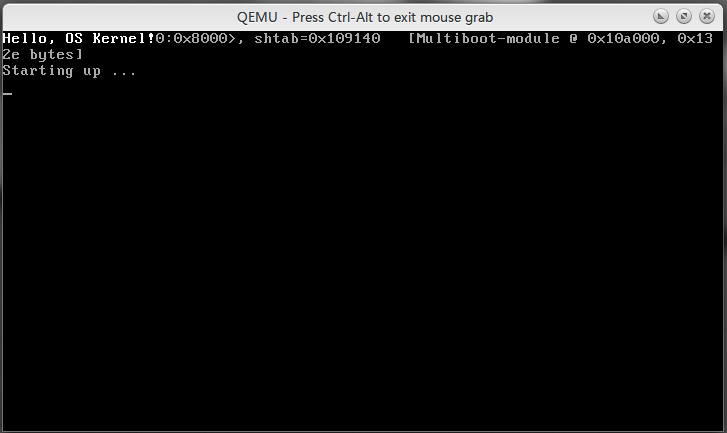
\includegraphics[scale=0.5]{picture/chapt3/hello_os_world.png}
      \caption{虚拟机里运行的 Hello, OS World!}
\end{figure}

\par 辛苦了这么久,终于看到一点点成功了。有没有一点小兴奋呢?下一章我们将完全的实现对屏幕的字符输出控制,并且有机会\allowbreak
的话我将把这个小内核运行在物理机上,和大家一起体验一下物理机运行的感觉。

\par 真正的好戏从下一章开始,别走开哦。

